\section{Evaluation}

We evaluate our method by comparing the reconstructed XYZ functions from our selected filters to the target XYZ functions, and computing the color difference $\Delta E$ under standard illuminants.
We use the Macbeth Color Checker \cite{Pascale2006RGBCO} as our test set, and evaluate under the D65 illuminant.
For each number of filters $N$, we compute the minimum $\Delta E$ across all combinations of $N$ filters from the Rosco Supergel set, and plot the relationship between $N$ and $\Delta E$.

\begin{center}
    \centering
    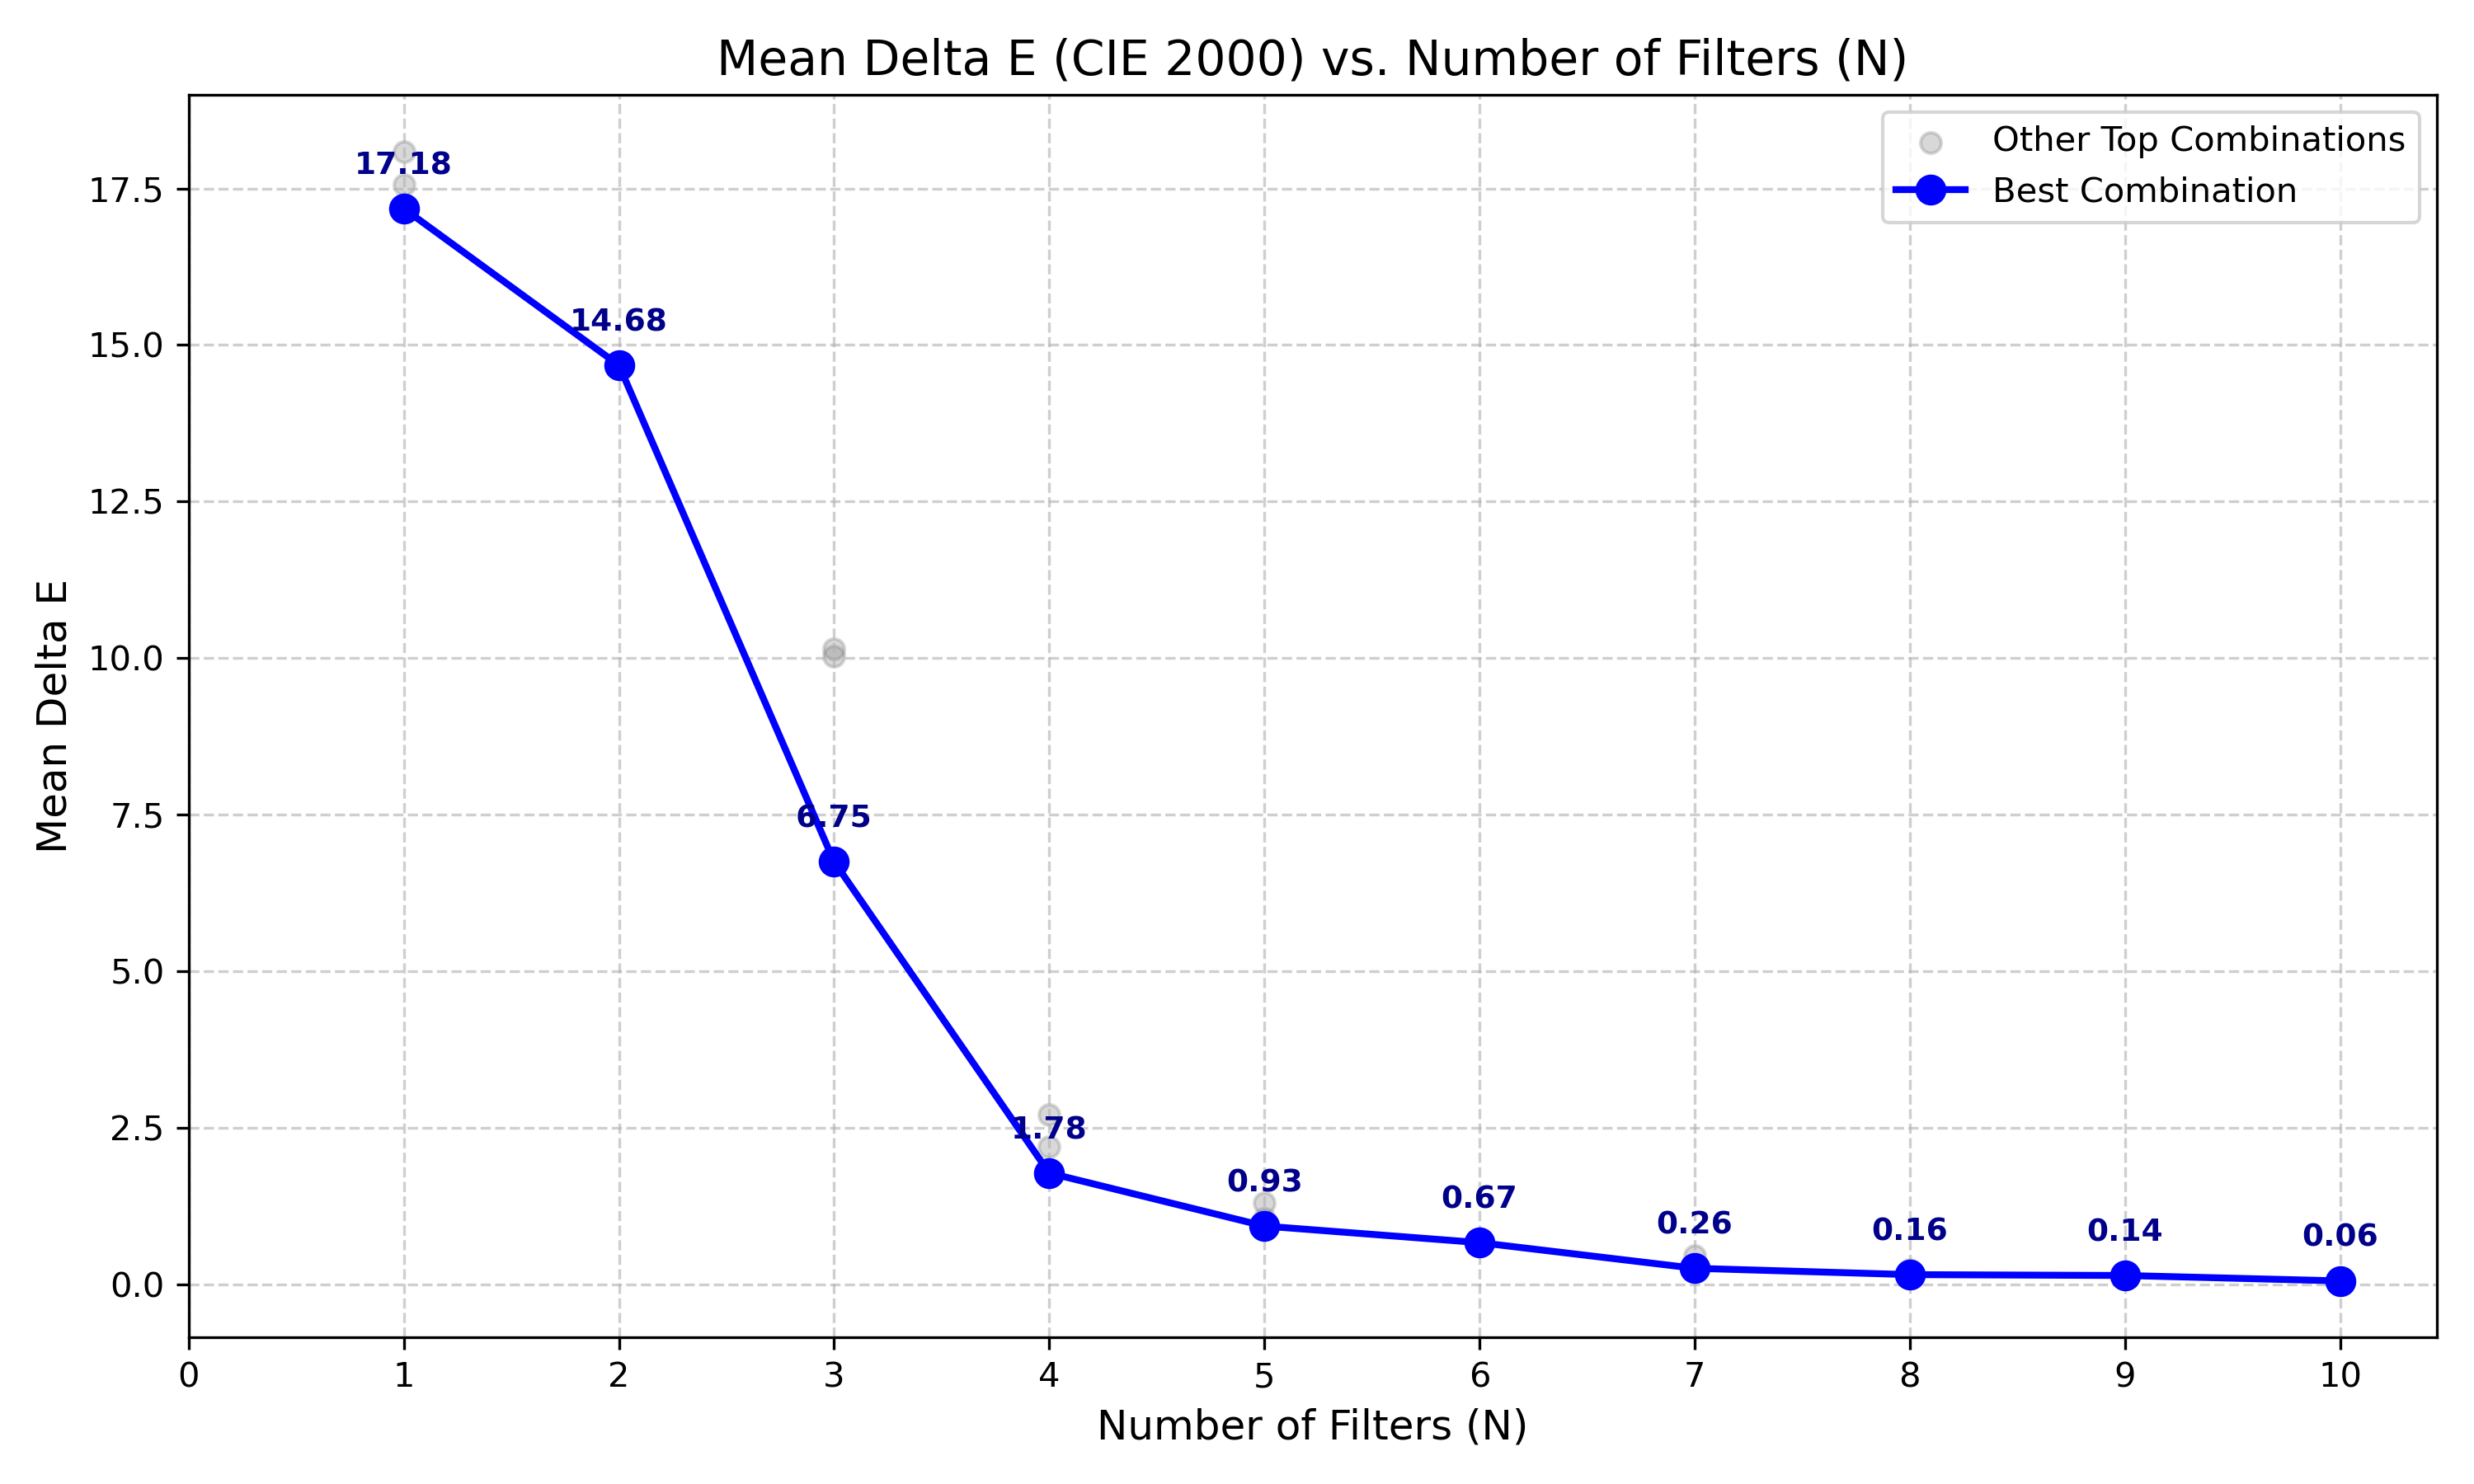
\includegraphics[width=.75\linewidth]{media/deltaE_vs_N_mse.png}
    \captionof{figure}{Best $\Delta E$ for each number of filters $N$ }
\end{center}

We also plot the resultant reconstructed XYZ functions for the best filter combination for various results at $N$ filters, and compare it to the target XYZ functions.
The $N=3$ case, we can see visible artifacts in the transmission functions. 
Note that the best MSE solution does not necessarily correspond to the best $\Delta E$ solution, and this is most evident at $N=3$ where the 3'rd best MSE achieves the low $\Delta E$ of 6.75.

\begin{center}
    \centering
    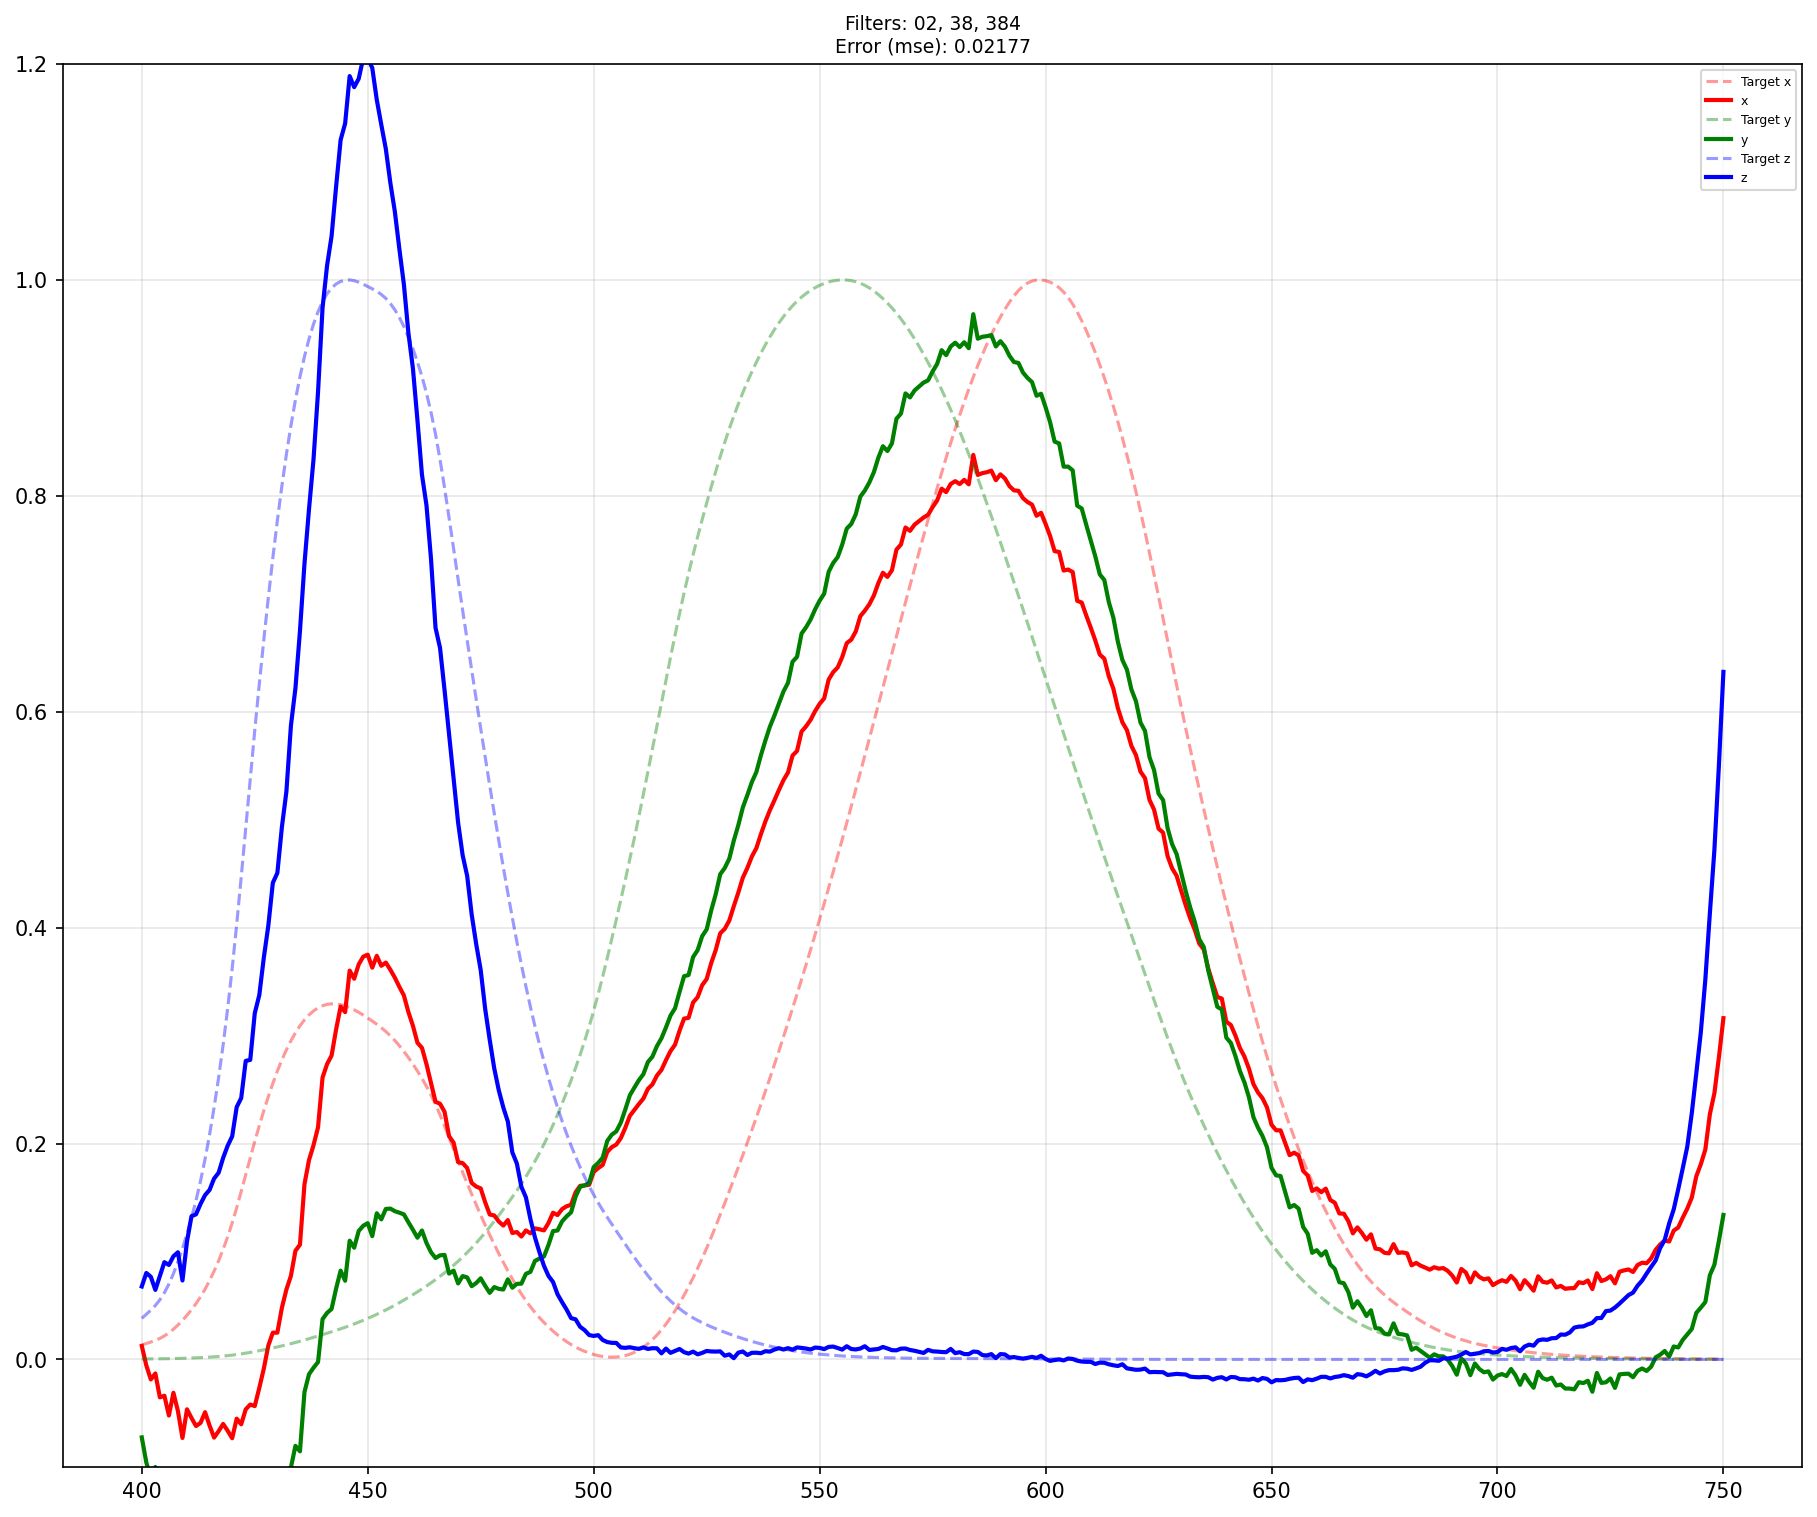
\includegraphics[width=.75\linewidth]{media/n3MSETransmission1.png}
    \captionof{figure}{Spectral Transmission for best XYZ Reconstruction for $N=3$ }
\end{center}

The best filter combination for $N=3$  achieves a $\Delta E$ of 6.7, which is above the just noticeable difference threshold of 2.3, indicating that the reconstructed colors may be distinguishable from the target colors under certain conditions.

\begin{center}
    \centering
    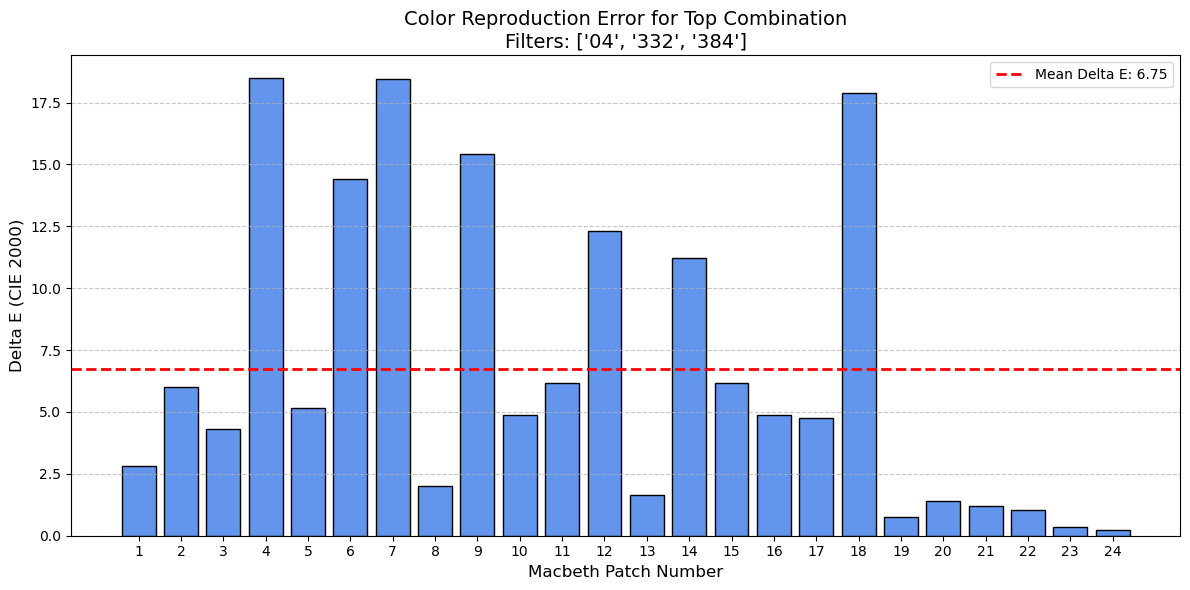
\includegraphics[width=.75\linewidth]{media/n3MSEbarRank2.png}
    \captionof{figure}{Best $\Delta E$ for each number of filters $N=3$ }
\end{center}

However, $N=4$ achieves a $\Delta E$ of 1.7, which is below the just noticeable difference threshold, indicating that the reconstructed colors are likely indistinguishable from the target colors under typical viewing conditions.

\begin{center}
    \centering
    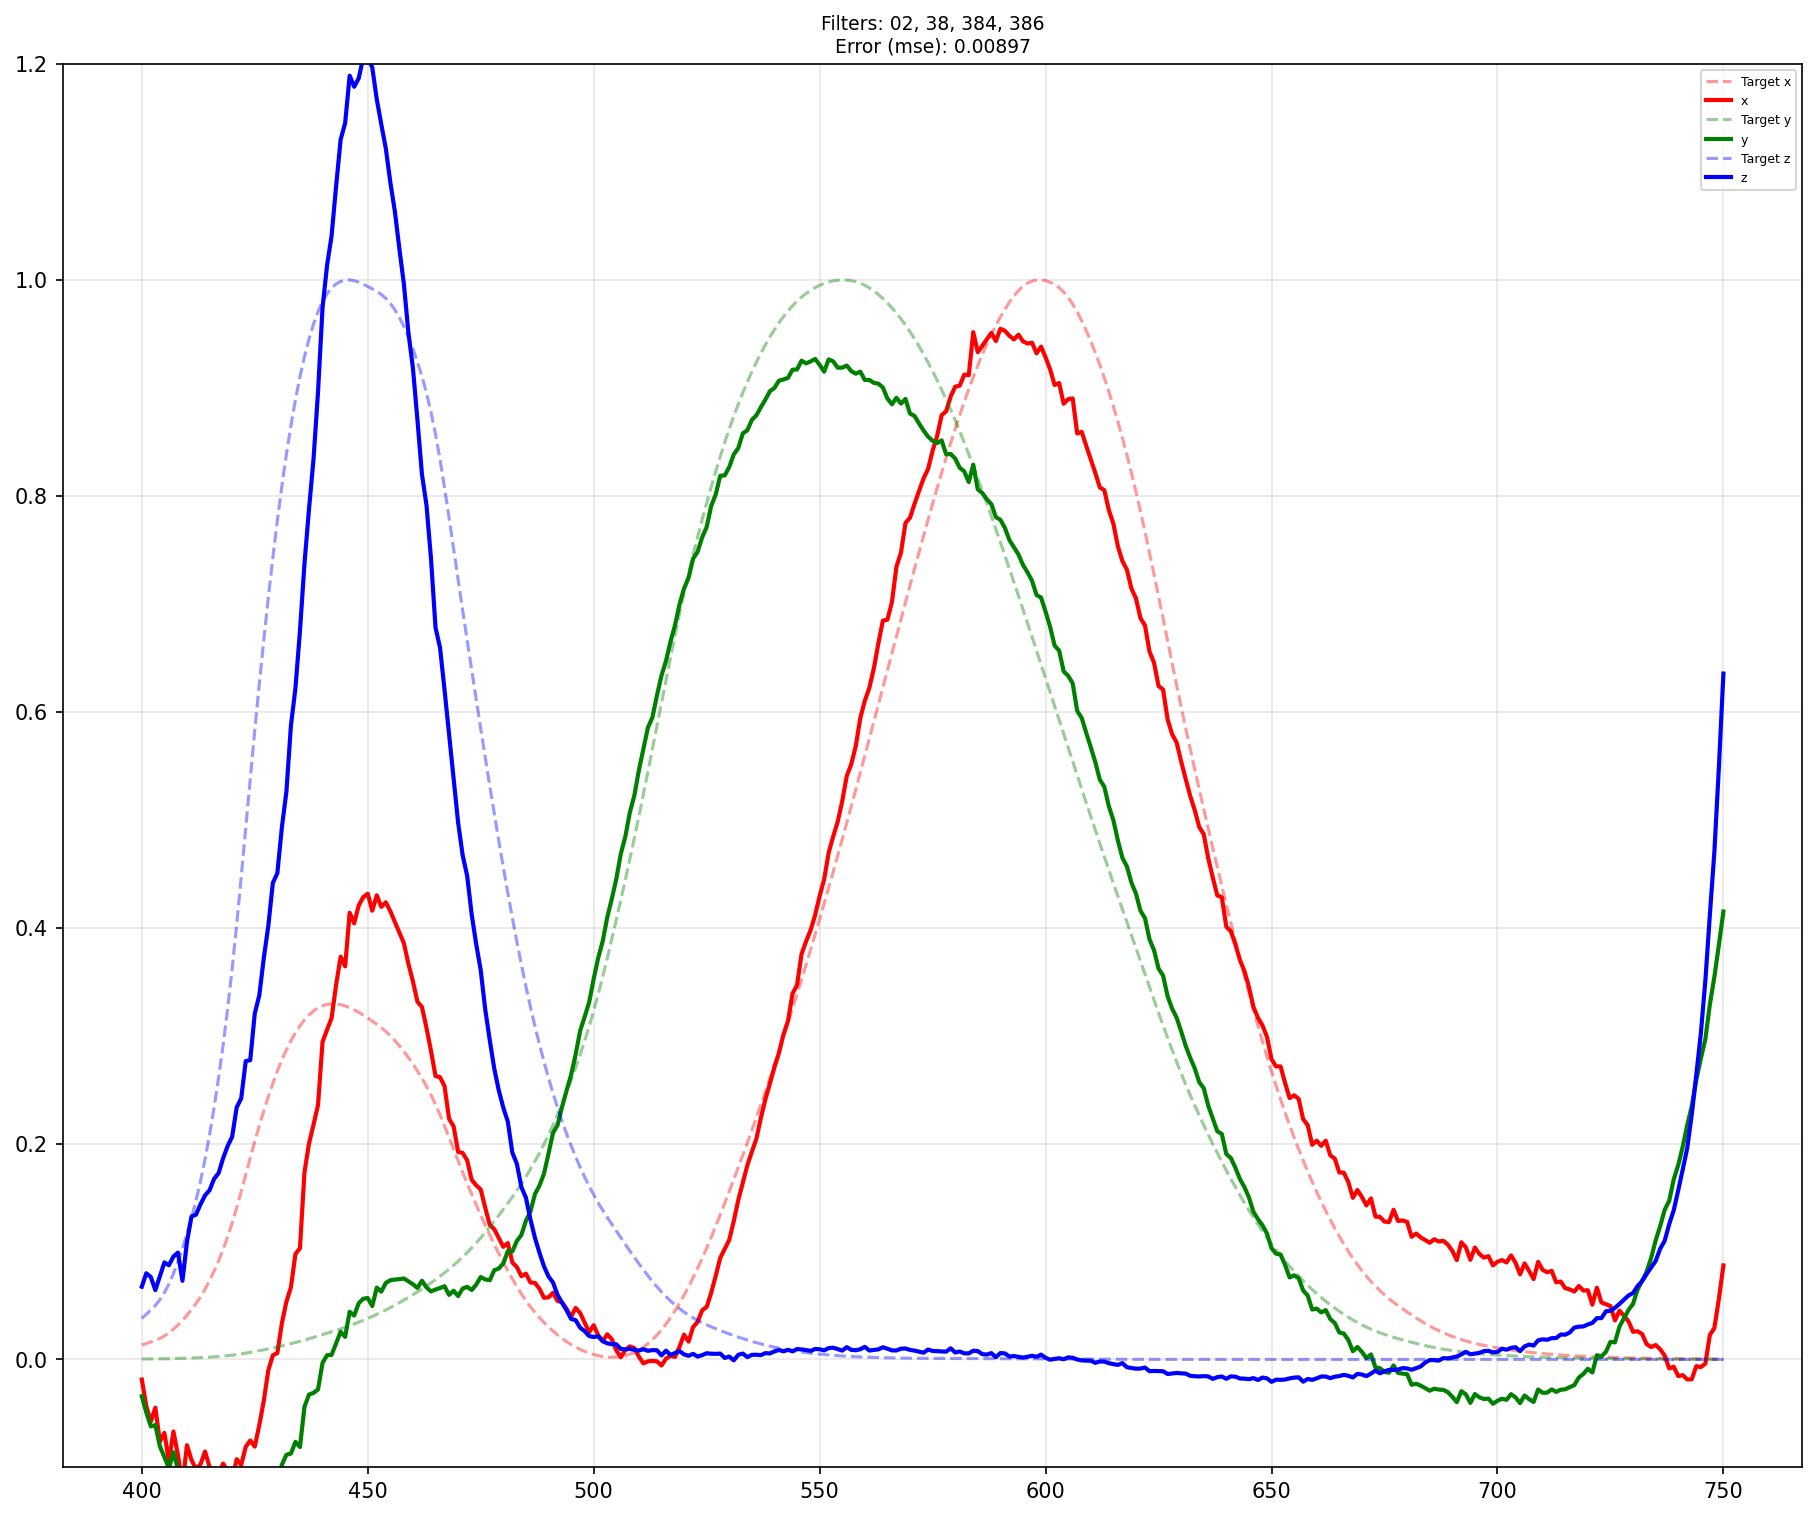
\includegraphics[width=.75\linewidth]{media/n4MSETransmission1.png}
    \captionof{figure}{Spectral Transmission for best XYZ Reconstruction for $N=4$ }
\end{center}
Further, $N=10$ achieves a $\Delta E$ of 0.08, virtually identical to the target patches. 


\begin{center}
    \centering
    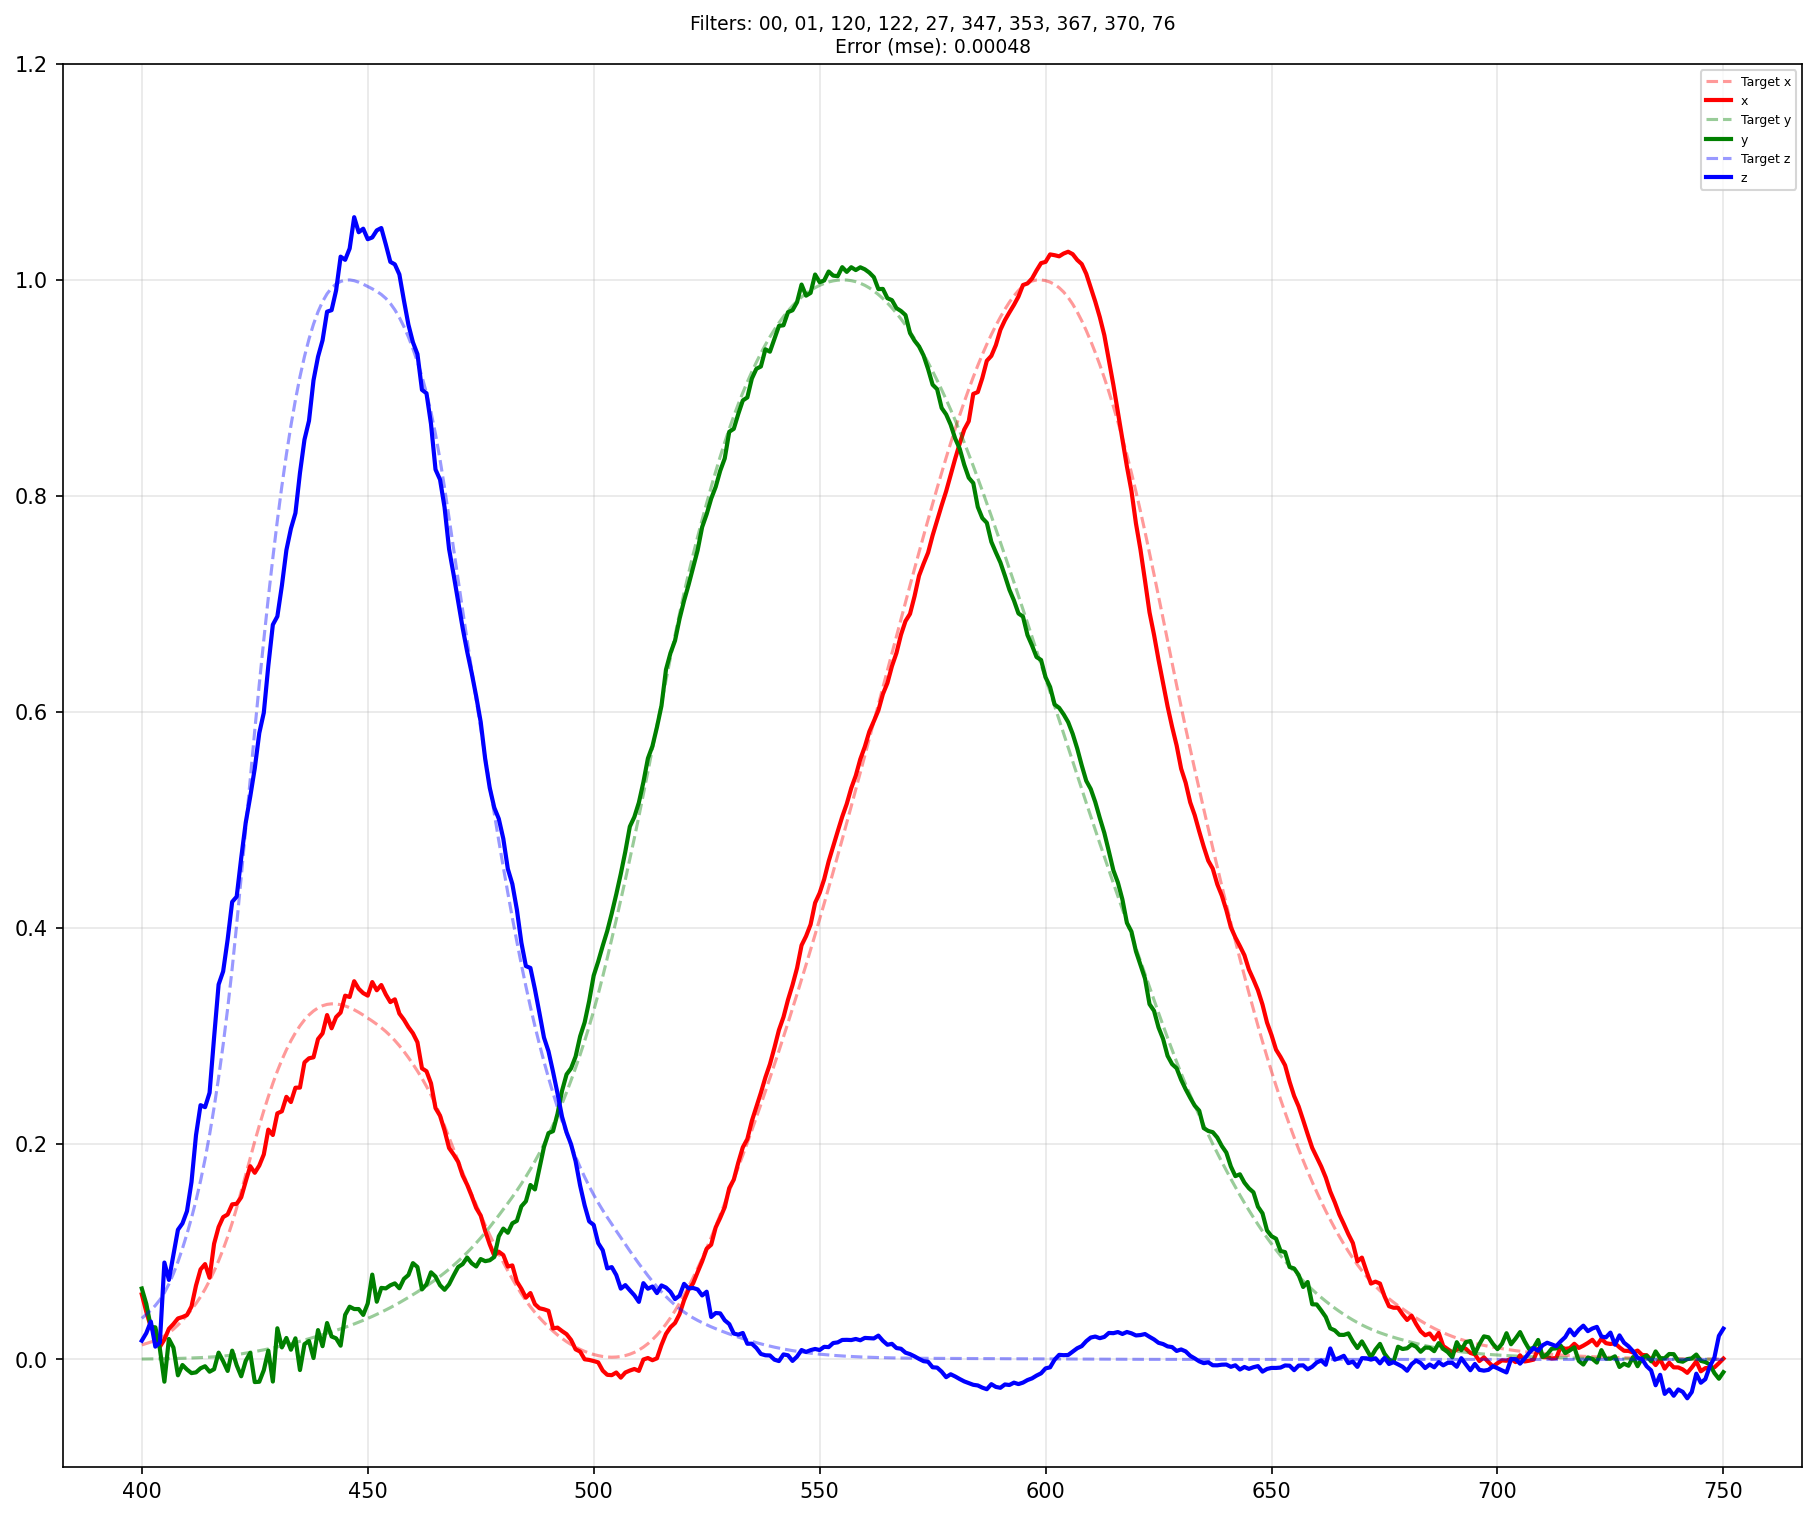
\includegraphics[width=.75\linewidth]{media/n10MSETransmission1.png}
    \captionof{figure}{Spectral Transmission for best XYZ Reconstruction for $N=10$ }
\end{center}

The distribution of $\Delta E$ across the 24 Macbeth Color Checker patches for the best filter combination for $N=10$ shows that all patches achieve a $\Delta E$ below 0.1.

\begin{center}
    \centering
    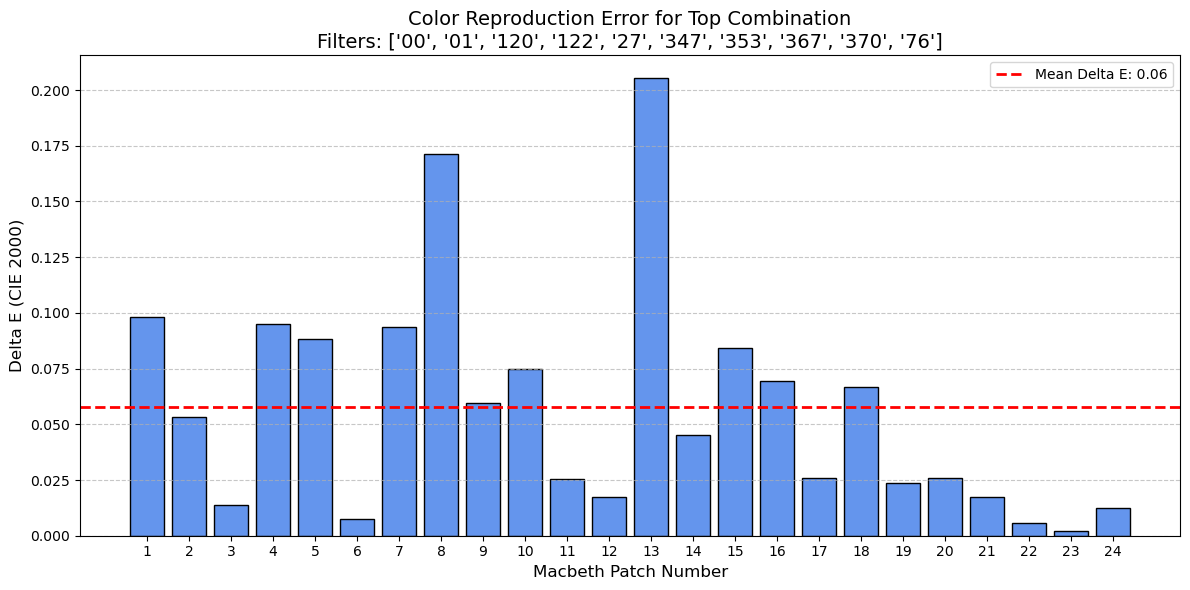
\includegraphics[width=.75\linewidth]{media/n10MSEbarRank0.png}
    \captionof{figure}{Best $\Delta E$ for each number of filters $N$ }
\end{center}

We show a render of the 24 Macbeth Color Checker patches under the D65 illuminant, reconstructed from the best filter combination for $N=10$, and compare it to the target Macbeth Color Checker render (upper left/lower right corners respectively). 

\begin{center}
    \centering
    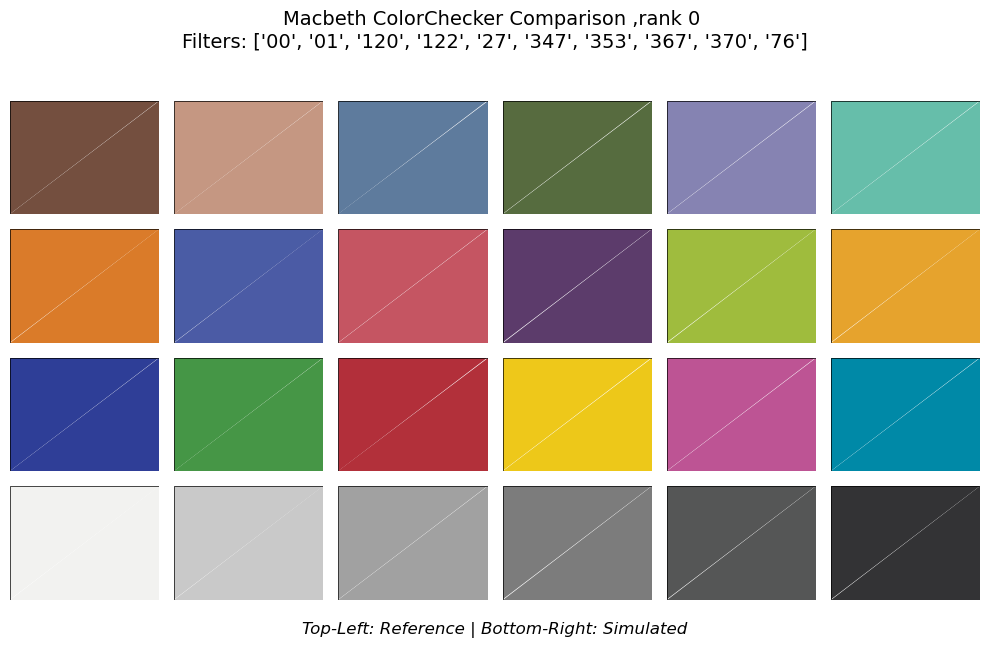
\includegraphics[width=.75\linewidth]{media/n10MacbethRank0.png}
    \captionof{figure}{Macbeth Color Checker Comparison for $N=10$ }
\end{center}

In addition, the $3 \times 10$ $\boldsymbol{M}$ matrix for the best $N=10$ reconstruction is shown below, displaying two important characteristics. 
First, all 10 filters are 'active' in at least one dimension at all times. 
\begin{center}
    \centering
    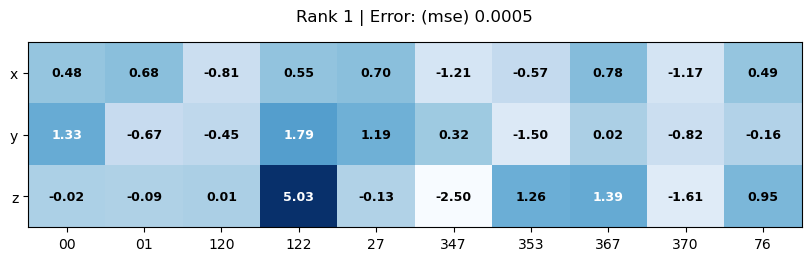
\includegraphics[width=\linewidth]{media/n10M.png}
    \captionof{figure}{$\boldsymbol{M}$ matrix for $N=10$ reconstruction}
\end{center}

